\let\negmedspace\undefined
\let\negthickspace\undefined
\documentclass[journal]{IEEEtran}
\usepackage[a5paper, margin=10mm, onecolumn]{geometry}
%\usepackage{lmodern} % Ensure lmodern is loaded for pdflatex
\usepackage{tfrupee} % Include tfrupee package

\setlength{\headheight}{1cm} % Set the height of the header box
\setlength{\headsep}{0mm}     % Set the distance between the header box and the top of the text

\usepackage{gvv-book}
\usepackage{gvv}
\usepackage{cite}
\usepackage{amsmath,amssymb,amsfonts,amsthm}
\usepackage{algorithmic}
\usepackage{graphicx}
\usepackage{textcomp}
\usepackage{xcolor}
\usepackage{txfonts}
\usepackage{listings}
\usepackage{enumitem}
\usepackage{mathtools}
\usepackage{gensymb}
\usepackage{comment}
\usepackage[breaklinks=true]{hyperref}
\usepackage{tkz-euclide} 
\usepackage{listings}
% \usepackage{gvv}                                        
\def\inputGnumericTable{}                                 
\usepackage[latin1]{inputenc}                                
\usepackage{color}                                            
\usepackage{array}                                            
\usepackage{longtable}                                       
\usepackage{calc}                                             
\usepackage{multirow}                                         
\usepackage{hhline}                                           
\usepackage{ifthen}                                           
\usepackage{lscape}
\begin{document}

\bibliographystyle{IEEEtran}
\vspace{3cm}

\title{NCERT-9.7.5}
\author{EE24BTECH11065 - Spoorthi yellamanchali
}
% \maketitle
% \newpage
% \bigskip
{\let\newpage\relax\maketitle}

\renewcommand{\thefigure}{\theenumi}
\renewcommand{\thetable}{\theenumi}
\setlength{\intextsep}{10pt} % Space between text and floats


\numberwithin{equation}{enumi}
\numberwithin{figure}{enumi}
\renewcommand{\thetable}{\theenumi}


\textbf{Question:}
\\
Form the differential equation of the family of circles in the first quadrant which touch the coordinate axes.
\\
\textbf{Solution: }
\\
The equation of a circle in the first quadrant, touching both the coordinate axes can be written as:
\begin{align}
    {\brak{x - r}}^2 + {\brak{y - r}}^2 = r^2;
\end{align}

where $r$ is the radius of the circle,\\
Let 
\begin{align}
    \frac{dy}{dx} = y^\prime
\end{align}
On differentiating both LHS and RHS of equation $\brak{0.1}$, we get,
\begin{align}
    2\brak{x - r} + 2\brak{y - r}\brak{\frac{dy}{dx}} = 0;
\end{align}
From this , we can write $r$ as ,
\begin{align}
    r = \frac{x + yy^\prime}{1 + y^\prime}
\end{align}
On substituting equation $\brak{0.5}$ in equation $\brak{0.1}$,i.e,on eliminating parameter $r$, we get,
\begin{align}
    {\left[x - \brak{\frac{x + yy^\prime}{1 + y^\prime}}\right]}^2 + {\left[y - \brak{\frac{x + yy^\prime}{1 + y^\prime}}\right]}^2 ={\brak{\frac{x + yy^\prime}{1 + y^\prime}}}^2 
    \end{align}
    \begin{align}
        {\left[\frac{\brak{x - y}y^\prime}{\brak{1 + y}^\prime}\right]}^2 + {\left[\frac{y - x}{\brak{1 + y}^\prime}\right]}^2 = {\left[\frac{x + yy^\prime}{\brak{1 + y^\prime}}\right]}^2
    \end{align}
    \begin{align}
         {\brak{x - y}}^2{y^\prime}^2 + {\brak{x - y}}^2 = {\brak{x + yy^\prime}}^2
    \end{align}
   \begin{align}
    \brak{x - y}^2\left[1 + \brak{y^\prime}^2\right] = \brak{x + yy^\prime}^2
\end{align}
On simplifying equation $\brak{0.8}$, we get,
\begin{align}
    \brak{y^\prime}^2\brak{x^2 - 2xy} - 2xyy^\prime + \brak{x - y}^2 - x^2 = 0
\end{align}
\begin{align}
    \brak{y^\prime}^2\brak{x^2 - 2xy} - 2xyy^\prime + \brak{y^2 - 2xy} = 0 
\end{align}
\begin{align}
     \brak{\frac{dy}{dx}}^2\brak{x^2 - 2xy} - 2xy\brak{\frac{dy}{dx}} + \brak{y^2 - 2xy} = 0 
\end{align}
$\therefore$ The differential equation of the family of circles touching the coordinate axes in the first quadrant is given by:
\begin{align}
    \brak{\frac{dy}{dx}}^2 - \brak{\frac{dy}{dx}}\brak{\frac{2xy}{x^2 - 2xy}} + \brak{\frac{y^2 - 2xy}{x^2 - 2xy}} = 0
\end{align}
It is a quadratic equation in terms of $\brak{\frac{dy}{dx}}$ in the form $at^2 + bt + c=0$,where, \\$a = 1$,$b =  \brak{\frac{2xy}{x^2 - 2xy}}$ and $c = \brak{\frac{y^2 - 2xy}{x^2 - 2xy}}$\\
On solving this to find the roots of the equation $\brak{0.12}$, we get an expression for $\frac{dy}{dx}$,
\begin{align}
    \frac{dy}{dx} = \frac{\brak{\frac{2xy}{x^2 - 2xy}} \pm \sqrt{\brak{\frac{2xy}{x^2 - 2xy}}^2 - 4\times\brak{\frac{y^2 - 2xy}{x^2 - 2xy}}}}{2}
\end{align}
\begin{align}
    \frac{dy}{dx} = \frac{y \pm \sqrt{\frac{2y}{x}\brak{x - y}^2}}{x - 2y} \\
    \frac{dy}{dx} = \frac{y \pm \sqrt{\frac{2y}{x}}\brak{x - y}}{x - 2y}
\end{align}
 we can see that,For given values of x,y,we get,two different values for $\frac{dy}{dx}$.\\
 For few points $\brak{x,y}$,two different circles are possible.\\
 for our plot,let, 
 \begin{align}
     \frac{dy}{dx} = \frac{y + \sqrt{\frac{2y}{x}}\brak{x - y}}{x - 2y}
 \end{align}
 
 From this differential equation,\\
 On assuming initial conditions $\brak{x_0,y_0}$, we get the equation and plot of a unique circle,\\
 Let us assume the initial conditions and on assuming a value for $h$ close to zero,we get,
 \begin{align}
     x_0 = 1\\
     y_0 = 2\\
     h = 0.01
 \end{align}
 Then , by the finite difference method which is a numerical technique for solving differential equations by approximating derivatives with differences.\\
The first forward difference approximation of the derivative of $f(x)$ at $x$ is given by: 
%This is forward difference, there are variations like backward difference, central differences also...
\begin{align}
    \frac{dy}{dx}=\frac{f(x+h)-f(x)}{h}      
\end{align}
Using this method we can write the expressions for $\brak{x_1,y_1}$ as :
\begin{align}
    x_1 = x_0 + h;
\end{align}
\begin{align}
  y_1 = y_0 + h\brak{\frac{dy}{dx}|_{x=x_0}}   
\end{align}
On substituting the expression of the derivative in equation $\brak{0.11}$, we get
\begin{align}
    y_1 = y_0 + h\left[\frac{y_0  + \sqrt{\frac{2y_0}{x_0}}\brak{x_0 - y_0}}{x_0 - 2y_0}\right]
\end{align}
On substituting the values of $x_0$,$y_0$ and $h$ in the above equations we get the point $\brak{x_1,y_1}$. \\
what we have essentially done above is, obtaining a point which is very close to the initial point along the direction of derivative at that point.\\
similarly we get, The difference equations for the curve,which are,
\begin{align}
     x_n = x_{n-1} + h 
\end{align}
\begin{align}
y_n = y_{n-1} + h\left[\frac{y_{n-1}  + \sqrt{\frac{2y_{n-1}}{x_{n-1}}}\brak{x_{n-1} - y_{n-1}}}{x_{n-1} - 2y_{n-1}}\right]
\end{align}
we can obtain points on the curve by using the above expressions for $y_n$ and $x_n$\\
 $\therefore$ we can plot the curve by the points obtained.
 \begin{figure}[h!]
   \centering
   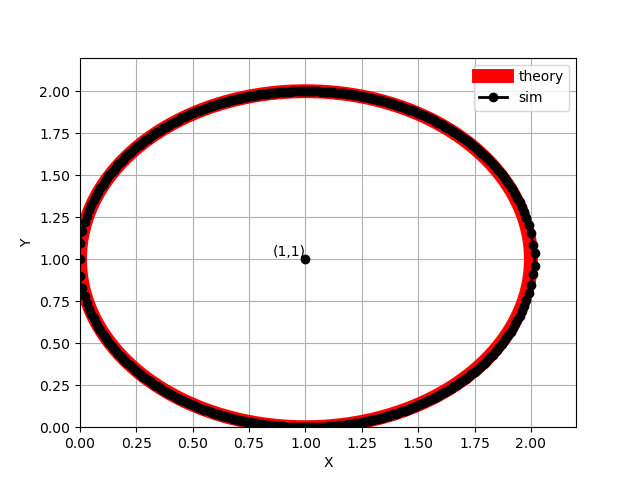
\includegraphics[width=0.75\columnwidth]{figures/Figure_1.png}
   \label{graph of the function}
\end{figure}
\end{document}


